\documentclass{beamer}
\usepackage[latin1]{inputenc}
%\usetheme{Montpellier}
%\usetheme{Boadilla}
%\usecolortheme[RGB={204,51,255}]{structure}
%\usecolortheme[named=purple]{structure}
\usecolortheme[RGB={128,62,62}]{structure}
%\definecolor{dark}{rgb}{0.3,0.15,0.3}
%\definecolor{light}{rgb}{0.8,0.6,0.8}
%\definecolor{reddish}{rgb}{.5,0.15,0.15}
\definecolor{dark}{rgb}{0.5,0.3,0.4}
%\definecolor{light}{rgb}{0.8,0.6,0.8}
\definecolor{reddish}{rgb}{.7,0.25,0.25}
\definecolor{greenish}{rgb}{.25,0.7,0.25}
\definecolor{blueish}{rgb}{.25,0.25,0.7}
\definecolor{purple}{rgb}{.5,0.0,0.5}
\usepackage{graphicx}
\usepackage{pstricks}

\usepackage{amssymb}

\usepackage{amsmath}
\setbeamertemplate{navigation symbols}{}

\newcommand{\crish}{\color{reddish}}
\newcommand{\cbla}{\color{black}}
\newcommand{\cred}{\color{red}}
\newcommand{\cblu}{\color{blue}}
\newcommand{\cgre}{\color{green}}

\newcommand{\sm}{\color{reddish}$}
\newcommand{\fm}{$\color{black}}
\usepackage{tikz}
\usetikzlibrary{arrows,decorations.markings,positioning}
\usepackage{epstopdf}
\title{Lecture 2: Combinatorics}
\author{COMS10014 Mathematics for Computer Science A}
\institute{\texttt{cs-uob.github.io/COMS10014/ and github.com/coms10011/2020\_21}}
\date{November 2020}
\begin{document}
\maketitle
\begin{frame}{Don't stop counting}
  Recall that \crish$P(A\cup B)=P(A)+P(B)$\cbla{}  if \crish$A\cap B=\emptyset$\cbla{}. In a discrete sample space an event can be written as the union of all the outcomes it contains, if \crish$$A=\{a_1,a_2,\ldots,a_k\}$$\cbla{}then
  \crish$$A=\{a_1\}\cup\{a_2\}\cup\ldots\cup\{a_k\}$$\cbla{}
  so
  \crish$$
  P(A)=P(\{a_1\})+P(\{a_2\})+\ldots+P(\{a_k\})  
  $$\cbla{}
\end{frame}

\begin{frame}{Don't stop counting}
  If all the probabilities are equal, say \crish$q$\cbla{} then, since \crish$P(X)=1$\cbla{}
  \crish$$
  q=\frac{1}{\#(X)}
  $$\cbla{}
  and
  \crish$$
  P(A)=\frac{\#(A)}{\#(X)}
  $$\cbla{}
  so to work out the probability we just need to calculate the number of points in \crish$A$\cbla{}.
\end{frame}

\begin{frame}{Simple example}
    \begin{center}
    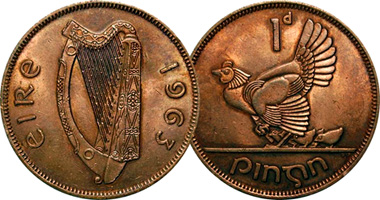
\includegraphics[width=3cm]{1d.jpg}
    \end{center}
A coin is flipped six times, what is the probability of getting all flips giving the same results? 
\end{frame}


\begin{frame}{Simple example}
    \begin{center}
    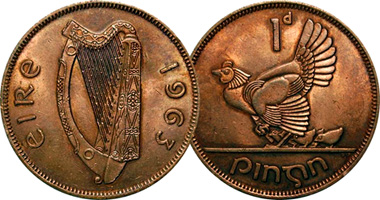
\includegraphics[width=3cm]{1d.jpg}
    \end{center}
    If a coin is flipped six times the set of outcomes looks like
    \crish$$X=\{HHHHHH,HHHHHT,HHHHTH,\ldots,TTTTTT\}$$\cbla{}
    The elements look like
    \crish$$\{ABCDEF\}$$\cbla{}
    where each element can be a \cblu$H$\cbla{} or a \cgre$T$\cbla{}
\end{frame}


\begin{frame}{Simple example}
    \begin{center}
    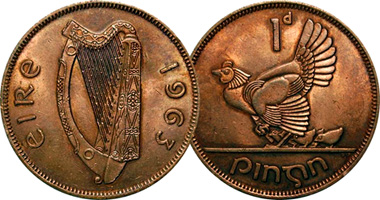
\includegraphics[width=3cm]{1d.jpg}
    \end{center}
    If a coin is flipped six times the set of outcomes looks like
    \crish$$X=\{HHHHHH,HHHHHT,HHHHTH,\ldots,TTTTTT\}$$\cbla{}
    The elements look like
    \crish$$\{\cblu{}H\crish{}BCDEF\}$$\cbla{}
    where each element can be a \cblu$H$\cbla{} or a \cgre$T$\cbla{}
\end{frame}


\begin{frame}{Simple example}
    \begin{center}
    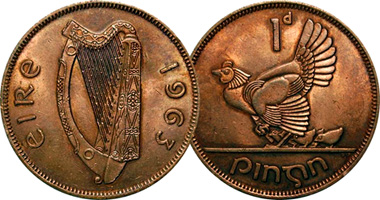
\includegraphics[width=3cm]{1d.jpg}
    \end{center}
    If a coin is flipped six times the set of outcomes looks like
    \crish$$X=\{HHHHHH,HHHHHT,HHHHTH,\ldots,TTTTTT\}$$\cbla{}
    The elements look like
    \crish$$\{\cgre{}T\crish{}BCDEF\}$$\cbla{}
    where each element can be a \cblu$H$\cbla{} or a \cgre$T$\cbla{}
\end{frame}


\begin{frame}{Simple example}
    \begin{center}
    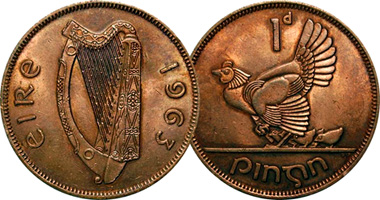
\includegraphics[width=3cm]{1d.jpg}
    \end{center}
    If a coin is flipped six times the set of outcomes looks like
    \crish$$X=\{HHHHHH,HHHHHT,HHHHTH,\ldots,TTTTTT\}$$\cbla{}
    The elements look like
    \crish$$\{A\cblu{}H\crish{}CDEF\}$$\cbla{}
    where each element can be a \cblu$H$\cbla{} or a \cgre$T$\cbla{}
\end{frame}


\begin{frame}{Simple example}
    \begin{center}
    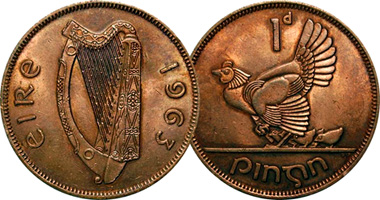
\includegraphics[width=3cm]{1d.jpg}
    \end{center}
    If a coin is flipped six times the set of outcomes looks like
    \crish$$X=\{HHHHHH,HHHHHT,HHHHTH,\ldots,TTTTTT\}$$\cbla{}
    The elements look like
    \crish$$\{A\cgre{}T\crish{}CDEF\}$$\cbla{}
    where each element can be a \cblu$H$\cbla{} or a \cgre$T$\cbla{}
\end{frame}


\begin{frame}{Simple example}
    \begin{center}
    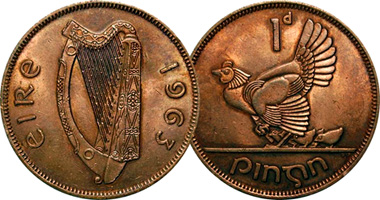
\includegraphics[width=3cm]{1d.jpg}
    \end{center}
    If a coin is flipped six times the set of outcomes looks like
    \crish$$X=\{HHHHHH,HHHHHT,HHHHTH,\ldots,TTTTTT\}$$\cbla{}
    The elements look like
    \crish$$\{AB\cblu{}H\crish{}DEF\}$$\cbla{}
    where each element can be a \cblu$H$\cbla{} or a \cgre$T$\cbla{}
\end{frame}


\begin{frame}{Simple example}
    \begin{center}
    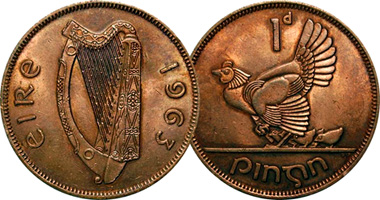
\includegraphics[width=3cm]{1d.jpg}
    \end{center}
    If a coin is flipped six times the set of outcomes looks like
    \crish$$X=\{HHHHHH,HHHHHT,HHHHTH,\ldots,TTTTTT\}$$\cbla{}
    The elements look like
    \crish$$\{AB\cgre{}T\crish{}DEF\}$$\cbla{}
    where each element can be a \cblu$H$\cbla{} or a \cgre$T$\cbla{}
\end{frame}


\begin{frame}{Simple example}
    \begin{center}
    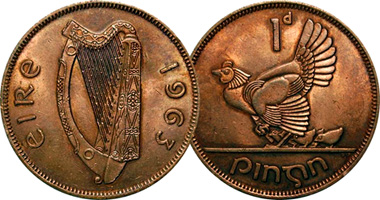
\includegraphics[width=3cm]{1d.jpg}
    \end{center}
    If a coin is flipped six times the set of outcomes looks like
    \crish$$X=\{HHHHHH,HHHHHT,HHHHTH,\ldots,TTTTTT\}$$\cbla{}
    so
    \crish$$\#(X)=2^6=64$$\cbla{}
\end{frame}

\begin{frame}{Simple example}
    \begin{center}
    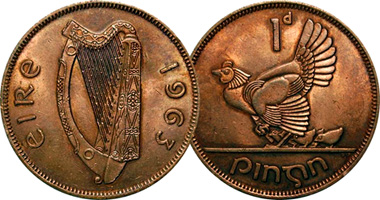
\includegraphics[width=3cm]{1d.jpg}
    \end{center}
    If a coin is flipped six times the set of outcomes looks like
    \crish$$X=\{HHHHHH,HHHHHT,HHHHTH,\ldots,TTTTTT\}$$\cbla{}
    so
    \crish$$\#(X)=2^6=64$$\cbla{}
    If \crish$S$\cbla{} is the event that all the outcomes are the same, it has just two elements:
    \crish$$S=\{HHHHHH,TTTTTT\}$$\cbla{}
    Hence
    \crish$$P(S)=\frac{\#(S)}{\#(X)}=\frac{1}{32}$$\cbla{}
\end{frame}

\begin{frame}{Combinatorics}
  \begin{center}
    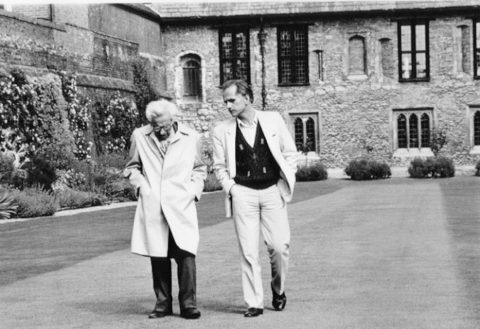
\includegraphics[width=6cm]{Bollobas-Erdos.png}
    \end{center}
  \begin{quote}
    The mathematics of counting things is called \textbf{combinatorics};
combinatorics is a rich area of mathematics with interesting links to
number theory and many applications in computer science.
  \end{quote}
  \vfill
  \flushright{\tiny{Paul Erd\"{o}s and B\'{e}la Bollab\'{a}s}}
  \end{frame}

\begin{frame}{The power set}
\crish$$
  A=\{a,b,c\}
$$\cbla{}
then the \textbf{power set} is
\crish$$
    \mathcal{P}(A)=\{\{\},\{a\},\{b\},\{c\},\{a,b\},\{b,c\},\{a,c\},\{a,b,c\}\}
$$\cbla{}
so
\crish$$
  \#(\mathcal{P}(A))=8
  $$\cbla{}
\end{frame}

\begin{frame}{The power set}
  In fact
  \crish$$  \#(\mathcal{P}(A))=2^{\#(A)}$$\cbla{}
  Consider a map from the power set to binary numbers where for a given subset you use ones for the element it contains and zeros for the ones it doesn't:
  \crish
  \begin{eqnarray*}
  \{\}&\leftrightarrow&000\cr
  \{a\}&\leftrightarrow&100\cr
  \{b\}&\leftrightarrow&010\cr
  &\ldots&\cr
  \{b,c\}&\leftrightarrow&011\cr
  \{a,b,c\}&\leftrightarrow&111
\end{eqnarray*}
  \cbla{}
  Hence the binary numbers of length \crish$\#(A)$\cbla{} count the elements of \crish$\mathcal{P}(A)$\cbla{}.
  \end{frame}

\begin{frame}{The factorial}
  The factorial
  \crish$$n!=n\times(n-1)\times\ldots\times 2 \times 1$$\cbla{}
  counts the number of different orders for \crish$n$\cbla{} objects. For example for \crish$\{a,b,c\}$\cbla{} there is
  \crish$$abc, bca, cab, acb, cba, bac$$\cbla{}
  \end{frame}


\begin{frame}{The factorial}
  There are \crish$n$\cbla{} choices of the first element:
  \crish$$\{\cblu{}a_1\crish{},a_2,a_3,\ldots,a_{n-1},a_n\}$$\cbla{}
  so
  \crish$$n!=\cblu{}n\crish{}\times\ldots{}$$\cbla{}
\end{frame}


\begin{frame}{The factorial}
  There are \crish$n$\cbla{} choices of the first element:
  \crish$$\{a_1,\cblu{}a_2\crish{},a_3,\ldots,a_{n-1},a_n\}$$\cbla{}
  so
  \crish$$n!=\cblu{}n\crish{}\times\ldots{}$$\cbla{}
\end{frame}


\begin{frame}{The factorial}
  There are \crish$n$\cbla{} choices of the first element:
  \crish$$\{a_1,a_2,\cblu{}a_3\crish{},\ldots,a_{n-1},a_n\}$$\cbla{}
  so
  \crish$$n!=\cblu{}n\crish{}\times\ldots{}$$\cbla{}
\end{frame}


\begin{frame}{The factorial}
  There are \crish$n$\cbla{} choices of the first element:
  \crish$$\{a_1,a_2,a_3,\ldots,\cblu{}a_{n-1}\crish{},a_n\}$$\cbla{}
  so
  \crish$$n!=\cblu{}n\crish{}\times\ldots{}$$\cbla{}
\end{frame}


\begin{frame}{The factorial}
  There are \crish$n$\cbla{} choices of the first element:
    \crish$$\{a_1,a_2,a_3,\ldots,a_{n-1},\cblu{}a_{n}\crish{}\}$$\cbla{}
  so
  \crish$$n!=\cblu{}n\crish{}\times\ldots{}$$\cbla{}
\end{frame}


\begin{frame}{The factorial}
  Then are \crish$n-1$\cbla{} choices of the second element:
    \crish$$\{\cblu{}a_1\crish,\cgre{}a_2\crish,a_3,\ldots,a_{n-1},a_{n}\}$$\cbla{}
  so
  \crish$$n!=\cblu{}n\crish{}\times\cgre{}(n-1)\crish\times\ldots{}$$\cbla{}
\end{frame}


\begin{frame}{The factorial}
  Then are \crish$n-1$\cbla{} choices of the second element:
    \crish$$\{\cblu{}a_1\crish,a_2,\cgre{}a_3\crish,\ldots,a_{n-1},a_{n}\}$$\cbla{}
  so
  \crish$$n!=\cblu{}n\crish{}\times\cgre{}(n-1)\crish\times\ldots{}$$\cbla{}
\end{frame}


\begin{frame}{The factorial}
  Then are \crish$n-1$\cbla{} choices of the second element:
    \crish$$\{\cblu{}a_1\crish,a_2,a_3,\ldots,\cgre{}a_{n-1}\crish,a_{n}\}$$\cbla{}
  so
  \crish$$n!=\cblu{}n\crish{}\times\cgre{}(n-1)\crish\times\ldots{}$$\cbla{}
\end{frame}

\begin{frame}{The factorial}
  Then are \crish$n-1$\cbla{} choices of the second element:
    \crish$$\{\cblu{}a_1\crish,a_2,a_3,\ldots,a_{n-1},\cgre{}a_n\crish\}$$\cbla{}
  so
  \crish$$n!=\cblu{}n\crish{}\times\cgre{}(n-1)\crish\times\ldots{}$$\cbla{}
and so on.
\end{frame}

\begin{frame}{Subsets of size $r$}
\crish$$
  A=\{a,b,c,d\}
$$\cbla{}
then the set of subsets of size two is
\crish$$
   [A]^2 =\{\{a,b\},\{a,c\},\{a,d\},\{b,c\},\{b,d\},\{c,d\}\}
$$\cbla{}
and
\crish$$
  \#([A]^2)=6
$$\cbla{}
where we are using \crish$[A]^r$\cbla{} for the set of subsets of \crish$A$\cbla{} of size \crish$r$\cbla.
\end{frame}

\begin{frame}{Subsets of size $r$}
  This works much the same as the factorial. If \crish$$\#(A)=n$$\cbla{}
  there are \crish$n$\cbla{} choices for the first element, then \crish$n-1$\cbla{} for the second. This time though there are only $r$ elements to pick, giving
  \crish$$n\times (n-1)\times \ldots (n-r+1)$$\cbla{}
  We can write this in terms of factorials
  \crish$$\frac{n\times (n-1)\times \ldots \times(n-r+1)\cblu\times (n-r)\times \ldots \times 1\crish}{\cblu{}(n-r)\times \ldots \times 1\crish}=\frac{n!}{(n-r)!}$$\cbla{}
  However we are overcounting, subsets don't care what order you pick them out in, so we need to divide by \crish$r!$\cbla{}:
  \crish$$\#([A]^r)=\frac{n!}{(n-r)!r!}$$\cbla{}
  \end{frame}


\begin{frame}{Subsets of size $r$}
  \crish$$\#([A]^r)=\frac{n!}{(n-r)!r!}$$\cbla{}
  This is just the binomial coefficient:
  \crish$$\#([A]^r)=\frac{n!}{(n-r)!r!}=\left(\begin{array}{c}n\\r\end{array}\right)={}_nC_r$$\cbla{}
\end{frame}

\begin{frame}{The binomial}
  The binomial coefficient appears in the binomial expansion:
  \crish$$  (x+y)^n=\sum_{r=0}^n \left(\begin{array}{c}n\\r\end{array}\right)x^ry^{n-r}$$\cbla{}
  We can use this to check our formulas make sense, clearly
\crish$$
  \mathcal{P}(A)=\emptyset\cup [A]^1\cup [A]^2\cup \ldots \cup [A]^n
$$\cbla{}
so we would expect
\crish$$
  2^n=\sum_{r=0}^n \left(\begin{array}{c}n\\r\end{array}\right)
$$\cbla{}
    and, in fact, that follows from the binomial examples with \crish$x=y=1$\cblu.
    \end{frame}
  
  

\end{document}
